\documentclass[11pt, spanish]{report}
\usepackage{Preamble}

\begin{document}

\begin{titlepage}

% a new command for the horizontal lines, change thickness
\newcommand{\HRule}{\rule{\linewidth}{0.5mm}}
%Center everything 
\center 

%	LOGO SECTION
% Logo of the university

\includegraphics[scale=0.25]{logo.jpg}\\[0.5cm]

%	HEADING SECTIONS
% Name of the university
\textsc{\LARGE Instituto Tecnologico de Buenos Aires}\\[0.5cm] 
% Name of the faculty
\textsc{\Large Ingeniera Electronica}\\[0.5cm] 
% Name of the department
\textsc{\Large Electronica III}\\[0.5cm] 

%	TITLE SECTION
\HRule \\[0.4cm]
% Title of the document
{\LARGE  Implementación de circuitos logicos}\\[0.2cm] 
\HRule \\[0.4cm]

%	AUTHOR SECTION
\begin{minipage}{0.4\textwidth}
\begin{flushleft} \large
\emph{Autores:}\\
Martín \textsc{Rodriguez Turco}
\\
Tobias \textsc{Scala}
\\
Guido \textsc{Panaggio}
\\
Juan Martin \textsc{Laguinge} 
\end{flushleft}
\end{minipage}
~
\begin{minipage}{0.4\textwidth}
\begin{flushright} \large
\emph{Profesores:} \\
Kevin \textsc{DeWald} % Supervisor's Name
\\
Pablo \textsc{Wundes} % Supervisor's Name
\\
Sebastian \textsc{Falconaro} % Supervisor's Name
\end{flushright}
\end{minipage}\\[6cm]

%	DATE SECTION
 % Date
{\large \today}\\[3cm]
 % Fill the rest of the page with whitespace
\vfill 

\end{titlepage}

% Table of Contents

\tableofcontents
 
\newpage

% Abstract
\phantomsection

\newpage

\clearpage
\chapter*{1-Control de la Activaci\'on de 2 Bombas de Agua}
\section{Objetivo}
El objetivo es implementar una máquina de estados el cual controle la activación de 2 bombas de agua denominados com B1 y B2 que controlen el nivel de agua de un dep\'osito el cual dispone de 2 sensores, uno en la parte inferior (I) y otro en la parte superior (S).
Esta m\'aquina de estados debe prender las bombas en función del nivel del agua en el dep\'osito.
Si el dep\'osito esta vac\'io (I = S = 0), entonces se prenden las 2 bombas.
Si el dep\'osito esta lleno por la mitad (I = 1, S = 0), entonces las bombas se alternan en su trabajo.
Si el dep\'osito esta lleno (I = S = 1), entonces se apagan las 2 bombas.

\section*{Explicaci\'on y Desarrollo}
Teni\'endo en cuenta las especificaciones de la m\'aquina de estados, se procede a realizar el diagrama de estados del mismo. Sea realizará el mismo desarrollo implementando tanto una m\'aquina de Moore como de Mealy.

\subsection*{Diagrama de Estados}
El diagrama de estados para la m\'aquina de estados de Moore queda de la siguiente forma:
\begin{center}
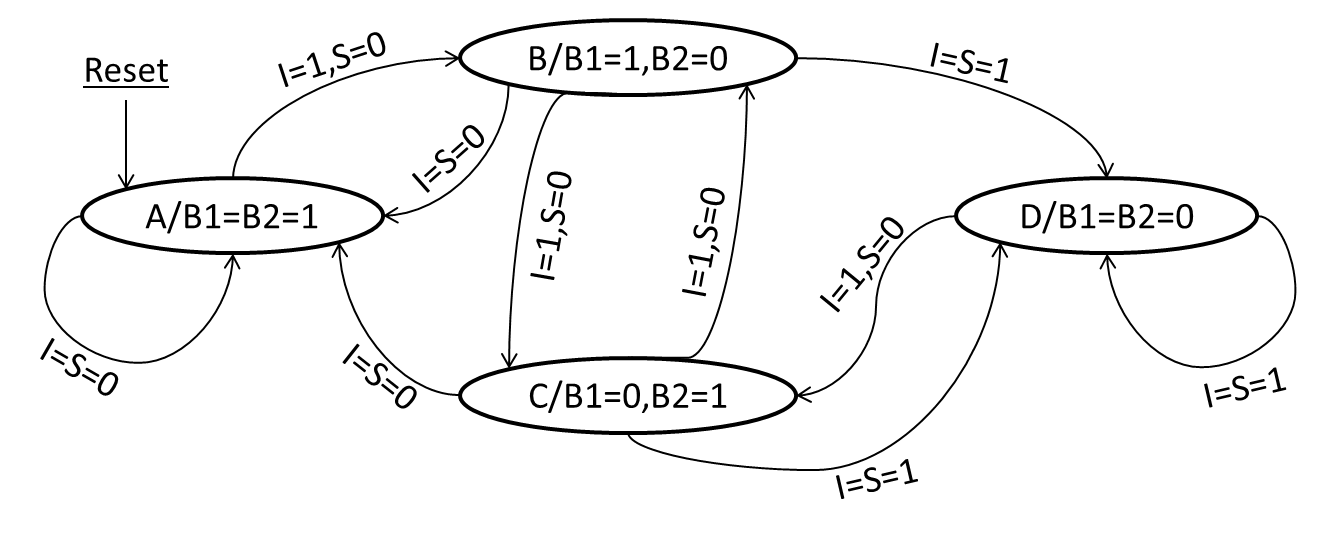
\includegraphics[scale=0.6]{../Ejercicio-1/moore1.png}
\end{center}
y la m\'aquina de estados de Mealy queda de la siguiente forma:
\begin{center}
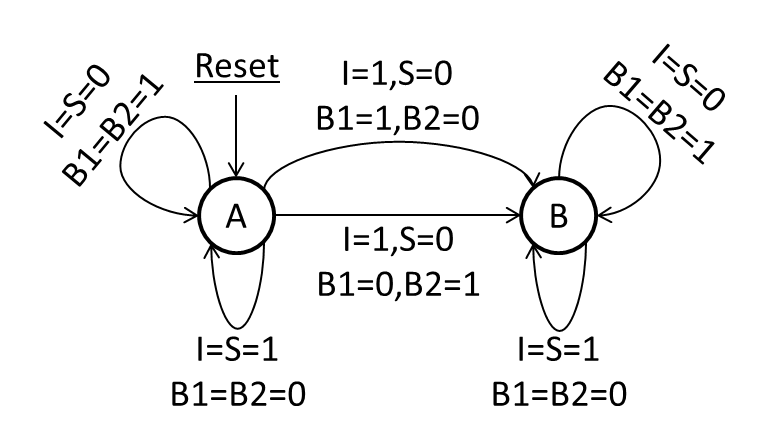
\includegraphics{../Ejercicio-1/mealy1.png}
\end{center}
Se puede ver que la mm\'aquina de estados de Mealy tiene menos estados que la de Moore ya que la salida depende de la entrada adem\'as del estado.

\subsection*{Tabla de Estados}
A partir de los diagramas de estados, se procede a armar las tablas de estados de cada m\'aquina. Asignando a los estados como: A = 00, B = 01, C = 10 y D = 11, la tabla de estados de Moore queda de la siguiente forma:\\
\begin{center}
	\begin{table}[h!]
		\begin{center}
			\caption{Tabla de Estados de Moore}
  			\begin{tabular}{|c|c|c|c|c|}
			    \hline
			    \multirow{2}{*}{Present State} &
			    \multicolumn{3}{c|}{Next State} &
			    \multirow{2}{*}{Output} \\
			    \cline{2-4} & 
			    I=S=0 & I=1,S=0 & I=S=1 & \\
			    \hline
			    y2 y1 & Y2 Y1 & Y2 Y1 & Y2 Y1 & B2 B1 \\
			    \hline
			    0 0 & 0 0 & 0 1 & x x & 1 1 \\
			    \hline
			    0 1 & 0 0 & 1 0 & 1 1 & 0 1 \\
			    \hline
			    1 0 & 0 0 & 0 1 & 1 1 & 1 0 \\
			    \hline
			    1 1 & x x & 1 0 & 1 1 & 0 0 \\
			    \hline
			\end{tabular}
		\end{center}
	\end{table}
\end{center}
Y asignando a los estados como: A = 0 y B = 1, la tabla de estados de Mealy queda de la siguiente forma:
\\
\begin{center}
	\begin{table}[h!]
		\begin{center}
			\caption{Tabla de Estados de Mealy}
  			\begin{tabular}{|c|c|c|c|c|c|c|}
			    \hline
			    \multirow{2}{*}{Present State} &
			    \multicolumn{3}{c|}{Next State} &
			    \multicolumn{3}{c|}{Output} \\
			    \cline{2-7} &
			    I=S=0 & I=1,S=0 & I=S=1 & I=S=0 & I=1,S=0 & I=S=1 \\
			    \hline
			    y & Y & Y & Y & B2 B1 & B2 B1 & B2 B1 \\
			    \hline
			    0 & 0 & 1 & 0 & 1 1 & 0 1 & 0 0 \\
			    \hline
			    1 & 1 & 0 & 1 & 1 1 & 1 0 & 0 0 \\
			    \hline
			\end{tabular}
		\end{center}
	\end{table}
\end{center}

\subsection*{Mapas de Karnaugh}
A continuaci\'on se procede a obtener las ecuaciones l\'ogicas de cada tabla de estados.
Empezando con la tabla de estados de Moore, se obtiene:

Para Y1: \\
NOTA: a = S, b = I, c = y2 y d = y1. 
\\
\begin{center}
	\begin{Karnaugh}
	    \contingut{0,0,0,x,1,0,1,0,x,x,x,x,x,1,1,1}
	    \implicant{12}{10}{blue}
   		\implicantcostats{4}{14}{green}
	\end{Karnaugh}
\end{center}
Donde se extrae que Y1 = S + y1*I.
\\
Para Y2: \\
NOTA: a = S, b = I, c = y2 y d = y1. 
\begin{center}
	\begin{Karnaugh}
		\contingut{0,0,0,x,0,1,0,1,x,x,x,x,x,1,1,1}
    	\implicant{12}{10}{blue}
	    \implicant{5}{15}{green}
	\end{Karnaugh}
\end{center}
Donde se extrae que Y2 = S + $\overline{y1}$*I.
\\
Para B1: \\
NOTA: a = y2, b = y1. 
\begin{center}
	\begin{Karnaughquatre}
		\contingut{1,1,0,0}
    	\implicant{0}{1}{blue}
	\end{Karnaughquatre}
\end{center}
Donde se extrae que B1 = $\overline{y2}$.
\\
Para B2: \\
NOTA: a = y2, b = y1. 
\begin{center}
	\begin{Karnaughquatre}
		\contingut{1,0,1,0}
    	\implicant{0}{1}{blue}
	\end{Karnaughquatre}
\end{center}
Donde se extrae que B2 = $\overline{y1}$.
\\
Y con estas ecuaciones ya es posible diseñar el circuito de Moore.
Ahora se obtendr\'an las ecuaciones l\'ogicas a partir de la tabla de estados de Mealy:

Para Y: \\
NOTA: a = y, b = S, c = I. 
\begin{center}
	\begin{Karnaughvuit}
		\contingut{0,1,x,0,1,0,x,1}
    	\implicant{7}{6}{blue}
    	\implicant{1}{red}
   		\implicantcostats{6}{4}{green}
	\end{Karnaughvuit}
\end{center}
Donde se extrae que Y = $\overline{S}$*I*$\overline{y}$ + y*(S + $\overline{I}$).
\\
Para B1: \\
NOTA: a = y, b = S, c = I. 
\begin{center}
	\begin{Karnaughvuit}
		\contingut{1,1,x,0,1,0,x,0}
    	\implicant{0}{1}{blue}
   		\implicantcostats{0}{6}{green}
	\end{Karnaughvuit}
\end{center}
Donde se extrae que B1 = $\overline{y}$*$\overline{s}$ + $\overline{I}$.
\\
Para B2: \\
NOTA: a = y, b = S, c = I. 
\begin{center}
	\begin{Karnaughvuit}
		\contingut{1,0,x,0,1,1,x,0}
    	\implicant{4}{5}{blue}
   		\implicantcostats{0}{6}{green}
	\end{Karnaughvuit}
\end{center}
Donde se extrae que B2 = y*$\overline{s}$ + $\overline{I}$.
Y con estas ecuaciones ya es posible diseñar el circuito de Mealy.

\section*{Circuitos L\'ogicos y Simulaci\'on en GTKWave}
Como ya se tiene lo necesario para diseñar y simular los circuitos, se los diseña quedando de la siguiente forma:
Circuito utilizando la m\'aquina de estados de Moore:
\begin{center}
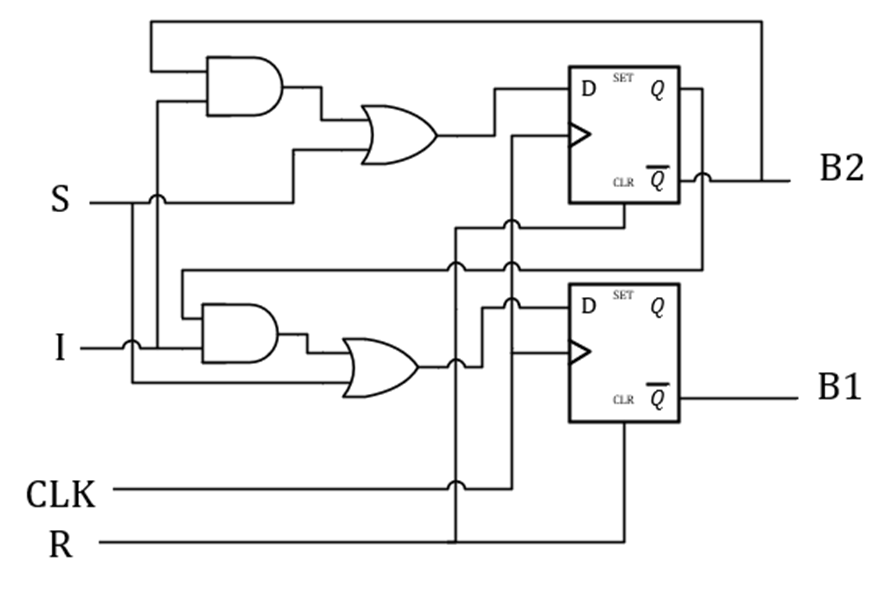
\includegraphics[scale=0.75]{../Ejercicio-1/moore3.png}
\end{center}
Al simular el circuito en GTKWave se obtiene lo siguiente:
\begin{center}
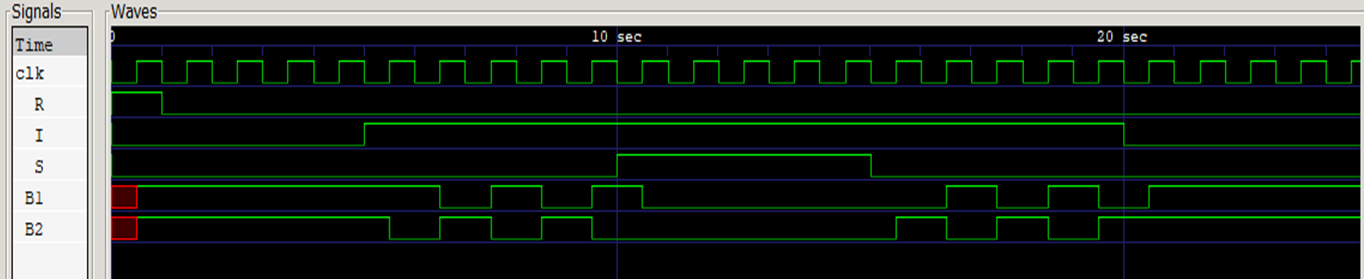
\includegraphics[scale=0.5]{../Ejercicio-1/moore2.png}
\end{center}
Circuito utilizando la m\'aquina de estados de Mealy:
\begin{center}
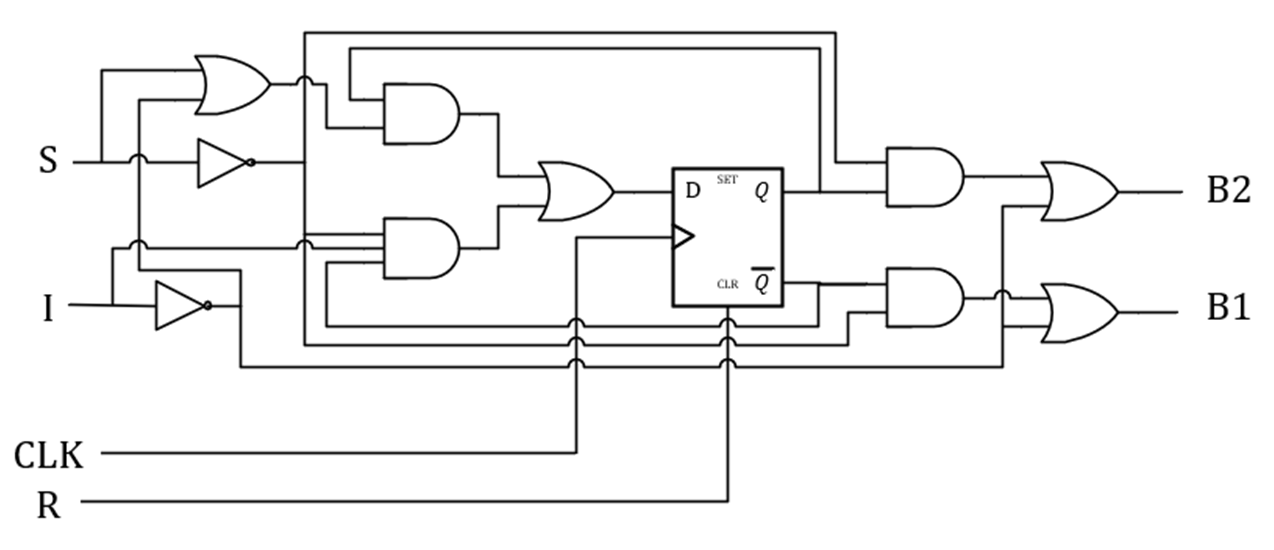
\includegraphics[scale=0.6]{../Ejercicio-1/mealy3.png}
\end{center}
Al simular el circuito en GTKWave se obtiene lo siguiente:
\begin{center}
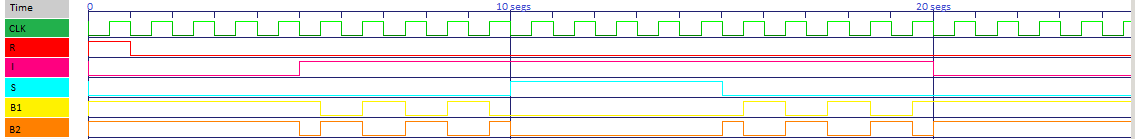
\includegraphics[scale=0.5]{../Ejercicio-1/mealy2.png}
\end{center}
La gran diferencia que se puede observar en la simulación es que la salidas est\'an desplasadas entre s\'i exactamente un ciclo de clock. Eso se debe a que el circuito el cual fue implimentado con Mealy responde m\'as r\'apido ya que su salida depende tanto de la entrada como del estado. En cambio el circuito el cual fue implementado con Moore solo depende del estado.
\chapter{Ejercicio 2}
Se desea diseñar una máquina de estados que, al recibir la siguiente secuencia de bits en forma sincrónica 1-1-0-1 encienda una salida y en caso contrario, la mantiene apagada. Se obtienen 5 estados para la misma, en los cuales va a haber un default que va a ser el estado al cual todos los demás estados van a volver en caso de no recibir los deseados además de ser el estado por el cual va a empezar la máquina de estados.\\
Podemos representar los mismos en el siguiente diagrama de estados:\\
\begin{figure}[h!]
	\label{f:Moore}
	\centering
	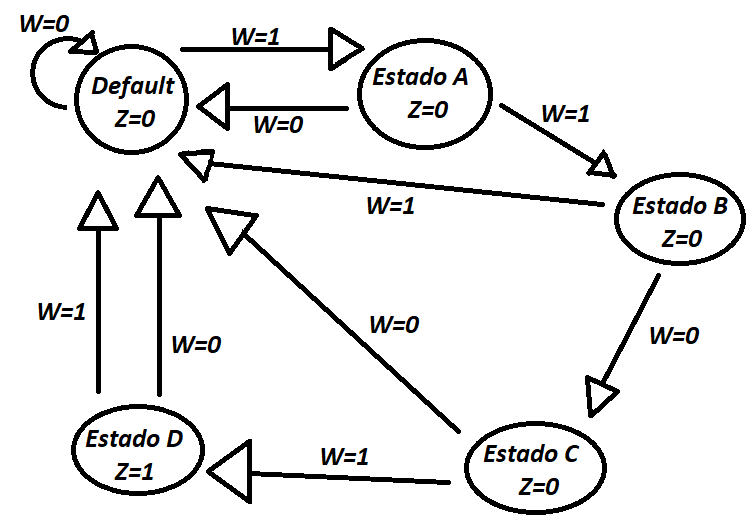
\includegraphics[scale=0.4]{../Ejercicio-2/Diagrama_de_estados.png}
	\caption{Diagrama de estados}
\end{figure}
En donde Z es la salida dada por la máquina de estados al encontrarse en el estado correspondiente y W es la entrada necesaria para que transicione al siguiente estado y la flecha es la encargada de indicar el sentido de la transición.\\
En este mismo esquema también queda encapsulado en la siguiente tabla de estados:\\
\FloatBarrier
\begin{table}[h!]
	\begin{center}
		\caption{Tabla de estados}
			\begin{tabular}{|c|c c|c|}
			\hline
			\textbf{Estado} &\multicolumn{2}{|c|}{Estado siguiente} & \textbf{Salida}\\
			\textbf{actual} & \textbf{ W=0 } & \textbf{ W=1 } & \textbf{Z}\\
			\hline
			\textbf{Default} & \textbf{ Default } & \textbf{ A } & 0\\
			\hline
			\textbf{A} & \textbf{ Default } & \textbf{ B } & 0\\
			\hline
			\textbf{B} & \textbf{ C } & \textbf{Default } & 0\\
			\hline
			\textbf{C} & \textbf{ Default } & \textbf{ D } & 0\\
			\hline
			\textbf{D} & \textbf{Default } & \textbf{Default} & 1\\
			\hline
			\end{tabular}
	\end{center}
\end{table}
\FloatBarrier
Para la implementación de esté falta realizar la asignación de valores de estado, lo cual nos lleva cambiar la tabla anterior por la siguiente:\\
\FloatBarrier
\begin{table}[h!]
	\begin{center}
		\label{t:Tabla}
		\caption{Tabla de estados asignados}
			\begin{tabular}{|c|c|c c|c|}
			\hline
			\textbf{Estado} & \textbf{Asignacion del} &\multicolumn{2}{|c|}{Estado siguiente} & \textbf{Salida}\\
			\textbf{actual}  & \textbf{Estado actual} & \textbf{ W=0 } & \textbf{ W=1 } & \textbf{Z}\\
			\hline
			\textbf{Default} & 000 & 000 &  001 & 0\\
			\hline
			\textbf{A} & 001 & 000 &  010 & 0\\
			\hline
			\textbf{B} & 010 & 011 & 000 & 0\\
			\hline
			\textbf{C} & 011 & 000 & 100 & 0\\
			\hline
			\textbf{D} & 100 & 000 & 000 & 1\\
			\hline
			\end{tabular}
	\end{center}
\end{table}
\FloatBarrier
%Empieza la parte de la maquina de Moore
\section{Máquina de Moore}
Para nuestro caso tenemos el siguiente circuito secuencial genérico:\\
\FloatBarrier
\begin{figure}[h!]
	\centering
	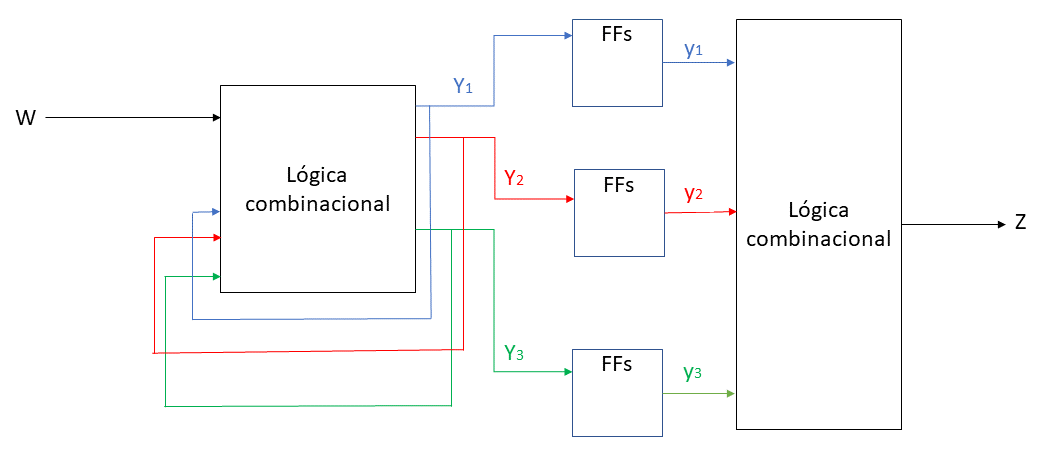
\includegraphics[scale=0.4]{../Ejercicio-2/Maquina_Moore.png}
	\caption{Circuito generico}
\end{figure}
\FloatBarrier
Donde vamos a utilizar Flip-Flops D dado que la entrada D de estos va a corresponder con el estado siguiente $Y_i$ y van a estar seteados por el clock para que esta salida luego cambia la variable $y_i$ a $Y_i$, dado que $y_i$ son las variables de estado actual.De la tabla \ref{t:Tabla}, obtenemos los siguientes mapas de Karnaugh:\\
\begin{center}
	\begin{figure}[h!]
		\begin{minipage}{0.5\textwidth}
			\caption{Mapa de Karnaugh para $Y_1$}
			\centering
			\begin{Karnaugh}
				\contingut{0,0,1,0,0,X,X,X,1,0,0,0,0,X,X,X}
				\implicant{2}{6}{red}
				\implicant{8}{8}{red}
			\end{Karnaugh}
		\end{minipage}
		 \hspace{5mm}
		\begin{minipage}{0.5\textwidth}
			\caption{Mapa de Karnaugh para $Y_2$}
			\centering
			\begin{Karnaugh}
				\contingut{0,0,1,0,0,X,X,X,0,1,0,0,0,X,X,X}
				\implicant{2}{6}{red}
				\implicant{13}{9}{red}
			\end{Karnaugh}
		\end{minipage}
	\end{figure}
\end{center}
\begin{center}
	\begin{figure}[h!]
		\begin{minipage}{0.5\textwidth}
			\caption{Mapa de Karnaugh para $Y_3$}
			\centering
			\begin{Karnaugh}
				\contingut{0,0,0,0,0,X,X,X,0,0,0,1,0,X,X,X}
				\implicant{15}{11}{red}
			\end{Karnaugh}
		\end{minipage}
		 \hspace{5mm}
		\begin{minipage}{0.5\textwidth}
			\caption{Mapa de Karnaugh para Z}
			\centering
			\begin{Karnaughvuit}
				\contingut{0,0,0,0,1,X,X,X}
				\implicant{4}{6}{red}
			\end{Karnaughvuit}
		\end{minipage}
	\end{figure}
\end{center}
En donde las X representan los don't care y se les decidió dar un valor acorde al cual permiten la simplificación del circuito. Dando como resultado las siguientes ecuaciones:\\
\begin{center}
	$Y_1 = W \cdot \overline{ y_3 } \cdot \overline{ y_2} \cdot \overline{ y_1 } + \overline{ W } \cdot \overline{ y_1} \cdot y_2  $\\
	$Y_2 = W \cdot \overline{ y_2} \cdot  y_1  + \overline{ W } \cdot \overline{ y_1} \cdot y_2  $\\
	$Y_3 = W \cdot  y_2 \cdot  y_1   $\\
	$Z = y_3  $\\
\end{center}
Se realizo la correspondiente simulación en verilog, el cual nos da un comportamiento ideal del circuito, obteniendo el siguiente resultado:\\
\FloatBarrier
\begin{figure}[h!]
	\centering
	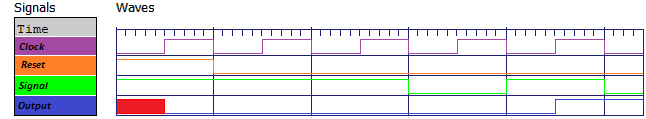
\includegraphics[scale=0.8]{../Ejercicio-2/Simulacion_Moore.png}
	\caption{Simulación}
\end{figure}
\FloatBarrier
%Empieza la parte de la maquina de Mealy
\section{Máquina de Mealy}
Para poder realizar la máquina de estados con el modelo de Mealy es necesario que la salida dependa tanto de los estados como de la entrada de esta, con lo cual van a ser necesarios realizar cambios a la actual máquina de estados.\\
Quitando el último estado del diagrama \ref{f:Moore} y expresando la salida junto con la entrada podemos obtener el siguiente diagrama:\\
\FloatBarrier
\begin{figure}[h!]
	\label{f:Meale}
	\centering
	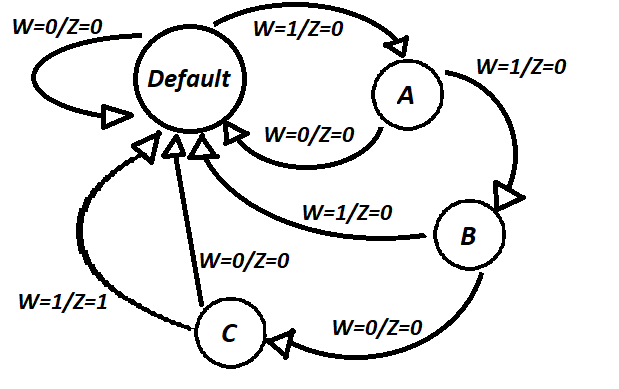
\includegraphics[scale=0.4]{../Ejercicio-2/Diagrama_de_estados_2.png}
	\caption{Diagrama de estados}
\end{figure}
\FloatBarrier
El diagrama tiene un estado menos ahorra, esto provoca los siguientes cambio en la tabla de asignación:\\
\FloatBarrier
\begin{table}[h!]
	\begin{center}
		\label{t:Tabla2}
		\caption{Tabla de estados asignados}
			\begin{tabular}{|c|c|c c|c|c|c|}
			\hline
			\textbf{Estado} & \textbf{Asignacion del} &\multicolumn{2}{|c|}{Estado siguiente} & \multicolumn{2}{|c|}{Salida Z}\\
			\textbf{actual}  & \textbf{Estado actual} & \textbf{ W=0 } & \textbf{ W=1 } & \textbf{ W=0 } & \textbf{ W=1 } \\
			\hline
			\textbf{Default} & 00 & 00 &  01 & 0 & 0\\
			\hline
			\textbf{A} & 01 & 00 &  10 & 0 & 0\\
			\hline
			\textbf{B} & 10 & 11 & 00 & 0 & 0\\
			\hline
			\textbf{C} & 11 & 00 & 00 & 0 & 1\\
			\hline
			\end{tabular}
	\end{center}
\end{table}
\FloatBarrier
La cual nos permite obtener los siguientes mapas de Karnaugh:\\
\begin{center}
	\begin{figure}[h!]
		\begin{minipage}{0.3\textwidth}
			\caption{Mapa de Karnaugh para $Y_1$}
			\centering
			\begin{Karnaughvuit}
				\contingut{0,0,1,0,1,0,0,0}
				\implicant{2}{2}{red}
				\implicant{4}{4}{red}
			\end{Karnaughvuit}
		\end{minipage}
		 \hspace{5mm}
		\begin{minipage}{0.3\textwidth}
			\caption{Mapa de Karnaugh para $Y_2$}
			\centering
			\begin{Karnaughvuit}
				\contingut{0,0,1,0,0,1,0,0}
				\implicant{2}{2}{red}
				\implicant{5}{5}{red}
			\end{Karnaughvuit}
		\end{minipage}
 		\hspace{5mm}
		\begin{minipage}{0.3\textwidth}
			\caption{Mapa de Karnaugh para Z}
			\centering
			\begin{Karnaughvuit}
				\contingut{0,0,0,0,0,0,0,1}
				\implicant{7}{7}{red}
			\end{Karnaughvuit}
		\end{minipage}
	\end{figure}
\end{center}
Dando como resultado de las simplificaciones las siguientes ecuaciones:\\
\begin{center}
	$Y_1 = W \cdot \overline{ y_2} \cdot \overline{ y_1 } + \overline{ W } \cdot \overline{ y_1} \cdot y_2  $\\
	$Y_2 = W \cdot \overline{ y_2} \cdot  y_1  + \overline{ W } \cdot \overline{ y_1} \cdot y_2  $\\
	$Z = W \cdot  y_2 \cdot y_1  $\\
\end{center}
Se realizo la correspondiente simulación en verilog, el cual nos da un comportamiento ideal del circuito, obteniendo el siguiente resultado:\\
\FloatBarrier
\begin{figure}[h!]
	\centering
	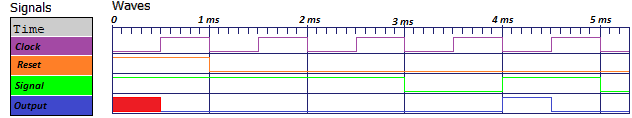
\includegraphics[scale=0.8]{../Ejercicio-2/Simulacion_Mealy.png}
	\caption{Simulación}
\end{figure}
\FloatBarrier

\chapter{Ejercicio 3}


\section{Consigna}

En este ejercicio se implementará una maquina de estados de Moore siguiendo lo solicitado por el trabajo y luego se hará una máquina de estados equivalente en su versión Mealy. Esta máquina es la que se muestra a continuación:\\

\begin{figure}[H]
\begin{center}
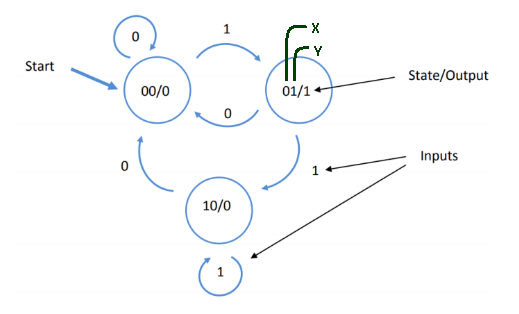
\includegraphics[scale=0.8]{../Ejercicio-3/imagenes/consigna.png}
\end{center}
\caption{Maquina de estados solicitada}

\end{figure}


\section{Maquina de estado de Moore}

Como se sabe las maquinas de estado de Moore se caracterizan por tener una salida unicamente dependiente del estado actual del sistema, sin depender de forma instantánea de la entrada.\\

Como primera instancia para resolución de esta máquina se define que valores para los bits denominados como \emph{X} e \emph{Y }, ilustrados en la figura anterior, caracterizan a cada uno de los estados, se puede observar ademas que cuando ambos de estos bits valen 1 la maquina no se encuentra en ningún estado relevante por lo que este se tratara como un estado de \emph{don\textasciiacute t care}. En la siguiente tabla se resume todo esto:\\

\begin{figure}[H]
\begin{centering}
\begin{tabular}{|c|c|c|}
\hline 
\multirow{2}{*}{Estados} & \multicolumn{2}{c|}{Condiciones}\tabularnewline
\cline{2-3} 
 & \multicolumn{1}{c|}{X} & Y\tabularnewline
\hline 
A & 0 & 0\tabularnewline
\hline 
B & 0 & 1\tabularnewline
\hline 
C & 1 & 0\tabularnewline
\hline 
\emph{don\textasciiacute t care} & 1 & 1\tabularnewline
\hline 
\end{tabular}
\par\end{centering}
\caption{Condiciones de estados}

\end{figure}

Una vez definido que valores identifican a cada uno de los estados lo que sigue es recopilar la información sobre como evoluciona el sistema según las entradas a este y como también cada estado determina la salida obtenida del sistema, todo esto se resume en la siguiente tabla:\\

\begin{figure}[H]
\begin{centering}
\begin{tabular}{|c|c|c|c|c|c|c|}
\hline 
\multicolumn{2}{|c|}{Estado Actual} & \multicolumn{4}{c|}{Estado futuro} & \multirow{3}{*}{Output}\tabularnewline
\cline{1-6} 
\multirow{2}{*}{x} & \multirow{2}{*}{y} & \multicolumn{2}{c|}{input = 0} & \multicolumn{2}{c|}{input = 1} & \tabularnewline
\cline{3-6} 
 &  & X & Y & X & Y & \tabularnewline
\hline 
0 & 0 & 0 & 0 & 0 & 1 & 0\tabularnewline
\hline 
0 & 1 & 0 & 0 & 1 & 0 & 1\tabularnewline
\hline 
1 & 0 & 0 & 0 & 1 & 0 & 0\tabularnewline
\hline 
1 & 1 & \emph{d} & \emph{d} & \emph{d} & \emph{d} & \emph{d}\tabularnewline
\hline 
\end{tabular}
\par\end{centering}
\caption{State assigned table}

\end{figure}

Nótese que se utilizaran letras minúsculas para designar estados actuales y letras mayúsculas para estados futuros.\\

Tanto la información sobre los estados futuros como de la salida se pueden contener en una tabla de verdad teniendo como variables los estados actuales \emph{x} e \emph{y} y el valor de entrada:\\

\begin{figure}[H]
\begin{centering}
\begin{tabular}{|c|c|c||c|c|}
\hline 
input & x & y & X & Y\tabularnewline
\hline 
\hline 
0 & 0 & 0 & 0 & 0\tabularnewline
\hline 
0 & 0 & 1 & 0 & 0\tabularnewline
\hline 
0 & 1 & 0 & 0 & 0\tabularnewline
\hline 
0 & 1 & 1 & 0 & 0\tabularnewline
\hline 
1 & 0 & 0 & 0 & 1\tabularnewline
\hline 
1 & 0 & 1 & 1 & 0\tabularnewline
\hline 
1 & 1 & 0 & 1 & 0\tabularnewline
\hline 
1 & 1 & 1 & \emph{d} & \emph{d}\tabularnewline
\hline 
\end{tabular}\ %
\begin{tabular}{|c|c||c|}
\hline 
x & y & Output\tabularnewline
\hline 
\hline 
0 & 0 & 0\tabularnewline
\hline 
0 & 1 & 1\tabularnewline
\hline 
1 & 0 & 0\tabularnewline
\hline 
1 & 1 & \emph{d}\tabularnewline
\hline 
\end{tabular}
\par\end{centering}
\caption{Tablas de verdad}

\end{figure}

Como se puede ver queda implícito en la tabla anterior que esta será una maquina de estado de Moore ya que la salida esta unicamente determinada por el estado actual.\\

Teniendo ya estas tablas de verdad se procede a utilizar el método de resolución con min-terminos del mapa de Karnaugh para obtener las expresiones lógicas de \emph{X} e \emph{Y} y de la salida, se
utilizarán los estados de \emph{don\textasciiacute t care} para lograr una expresión lo mas compacta posible, se aclara que \emph{y1} y \emph{y2} representan a \emph{x} e \emph{y} respectivamente mientras que W denota el valor de entrada:\\

\begin{figure}[H]
	\centering
	\begin{Karnaughvi}
		\contingut{0,0,0,X,0,1,1,X}
		\implicant{5}{7}{red}
		\implicant{7}{6}{green}
	\end{Karnaughvi}
\caption{Mapa de Karnaugh de X}
\end{figure}

\begin{figure}[H]
\centering
	\begin{Karnaughvi}
		\contingut{0,0,0,X,1,0,0,X}
		\implicant{4}{4}{red}
	\end{Karnaughvi}
\caption{Mapa de Karnaugh de Y}
\end{figure}

\begin{figure}[H]
\centering
	\begin{Karnaughquatre}
		\contingut{0,0,1,X}
		\implicant{2}{3}{red}
	\end{Karnaughquatre}

\caption{Mapa de Karnaugh de Output}
\end{figure}

Las expresiones obtenidas son las siguientes:\\
\begin{itemize}
\item $X=inp\cdot x+inp\cdot y=inp\cdot(x+y)$
\item $Y=inp\cdot\overline{x}\cdot\overline{y}$
\item $Output=y$
\end{itemize}
Las cuales describen el comportamiento del siguiente circuito:\\

\begin{figure}[H]
\begin{centering}
\includegraphics[scale=0.8]{../Ejercicio-3/\string"imagenes/E3 TP3 Moore\string".png}
\par\end{centering}
\caption{Circuito de Moore}
\end{figure}


\section{Maquina de estado de Mealy}

Mientras que la maquina de estados de Moore depende exclusivamente del estado actual del sistema la de Mealy no solo depende de este sino también del que se tiene a la entrada del sistema, de allí una de las principales diferencias con respecto a las maquinas de estado de Moore, un cambio a la entrada se verá reflejado \emph{instantáneamente} a la salida.\\

Para llegar a que la salida esté en relación directa con la entrada se analizó paso a paso el comportamiento del sistema. Se entiende que la maquina verá un 1 a su salida cuando se tenga un 1 a la entrada y simultaneamente se esté en un estado latente o inicial, una vez muestreado este valor se pasará a un nuevo estado en el cual el sistema arrojará 0 ante cualquier salida. En este estado se permanecerá mientras se siga leyendo un 1 a la entrada y se regresará al estado inicial en
caso contrario. A continuación un ejemplo:\\

\begin{figure}[H]
\begin{centering}
\begin{tabular}{|c|c|c|c|c|c|c|c|c|}
\hline 
 & $t_{0}$ & $t_{1}$ & $t_{2}$ & $t_{3}$ & $t_{4}$ & $t_{5}$ & $t_{6}$ & $t_{7}$\tabularnewline
\hline 
\hline 
Input & 0 & 1 & 0 & 1 & 1 & 1 & 0 & 1\tabularnewline
\hline 
Output & 0 & 1 & 0 & 1 & 0 & 0 & 0 & 1\tabularnewline
\hline 
\end{tabular}
\par\end{centering}
\caption{Ejemplo de funcionamiento de la maquina}

\end{figure}

Visto el comportamiento de la máquina se propone el siguiente esquema para este:\\

\begin{figure}[H]
\begin{centering}
\includegraphics[scale=0.8]{../Ejercicio-3/\string"imagenes/E3 TP3 Mealy paint\string".png}
\par\end{centering}
\caption{Esquema de la maquina de Mealy}

\end{figure}

Del mismo modo que antes se puede representar el funcionamiento de la maquina en la siguiente tabla:\\

\begin{figure}[H]
\begin{centering}
\begin{tabular}{|c|c|c|c|c|}
\hline 
\multirow{2}{*}{Estado actual} & \multicolumn{2}{c|}{Estado futuro} & \multicolumn{2}{c|}{Output}\tabularnewline
\cline{2-5} 
 & input = 0 & input = 1 & input = 0 & input = 1\tabularnewline
\hline 
A & A & B & 0 & 1\tabularnewline
\hline 
B & A & B & 0 & 0\tabularnewline
\hline 
\end{tabular}
\par\end{centering}
\caption{State assigned table}

\end{figure}

Como se ha planteado hasta ahora solo existen 2 estados posibles por lo tanto si se considera la variable \emph{estados} (la cual se llamara \emph{x} para los presentes y \emph{X} para los futuros) se puede
decir que esta nueva variable posee un valor binario, 0 para el estado A y 1 para el estado B. Desde aquí se puede implementar la siguiente tabla de verdad:\\

\begin{figure}[H]
\begin{centering}
\begin{tabular}{|c|c||c|c|}
\hline 
x & input & X & Output\tabularnewline
\hline 
\hline 
0 & 0 & 0 & 0\tabularnewline
\hline 
0 & 1 & 1 & 1\tabularnewline
\hline 
1 & 0 & 0 & 0\tabularnewline
\hline 
1 & 1 & 1 & 0\tabularnewline
\hline 
\end{tabular}
\par\end{centering}
\caption{Tablas de verdad}

\end{figure}

Desde aquí es fácil observar las siguientes implicaciones lógicas:\\
\begin{itemize}
\item $X=inp$
\item $Output=inp\cdot\overline{x}$
\end{itemize}
Las cuales se representan el funcionamiento del siguiente circuito:\\

\begin{figure}[H]
\begin{centering}
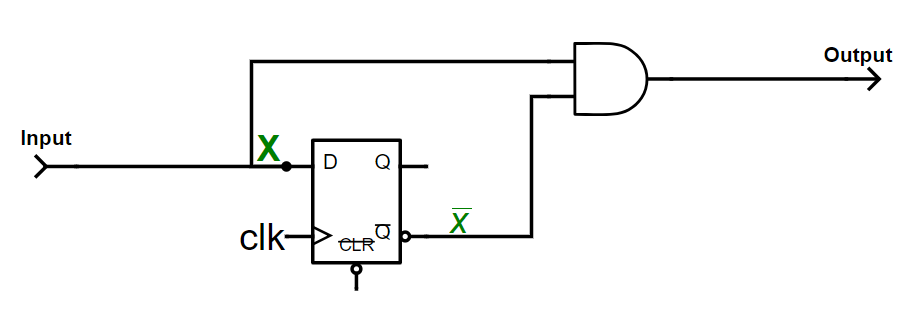
\includegraphics[scale=0.8]{../Ejercicio-3/imagenes/E3-TP3-Mealy.png}
\par\end{centering}
\caption{Circuito de Mealy}

\end{figure}

\section{Conversión de tensiones}

Una condición para el diseño de los circuitos es que estos reciban y devuelvan tensiones de 0 o 5V mientras que la lógica interna de esta debe operar a 3.3V, por lo que se deberá implementar tecnología que trabaje con este nivel de tensión realizando la respectiva conversión de voltaje tanto a la entrada como a la salida.\\

Para esto último se utilizó el circuito integrado SN7407N el cual permite realizar cómodamente una conmutación de tensión dado que se le permite al usuario operar con el colector del transistor ubicado a la salida de este, es decir, este es un dispositivo \emph{open-colector}. Un diagrama simplificado de su funcionamiento se muestra a continuación:\\

\begin{figure}[H]
\begin{centering}
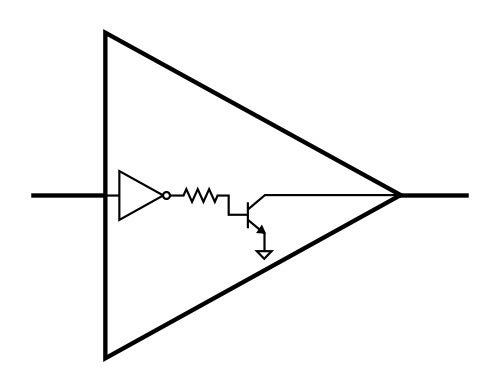
\includegraphics[scale=1.2]{../Ejercicio-3/imagenes/SN7407N.jpg}
\par\end{centering}
\caption{Diagrama del SN7407N}

\end{figure}

Como se puede ver un 1 lógico a la entrada dejara en alta impedancia la salida del integrado, dado que el transistor estará en estado de corte, con lo cual implementado una resistencia de pull-up sobre el colector a la salida se tendrá la tensión deseada.\\

\section{Resultados obtenidos}
Ya con los esquematicos y la estructura del circuito definida se procedio a realizar la implementación de esta. Finalmente el circuito se comportó conforme a lo esperado lo cual se muestra en las siguientes imagenes que se consideraron suficientemente representativas:\\

\begin{figure}[H]
\begin{centering}
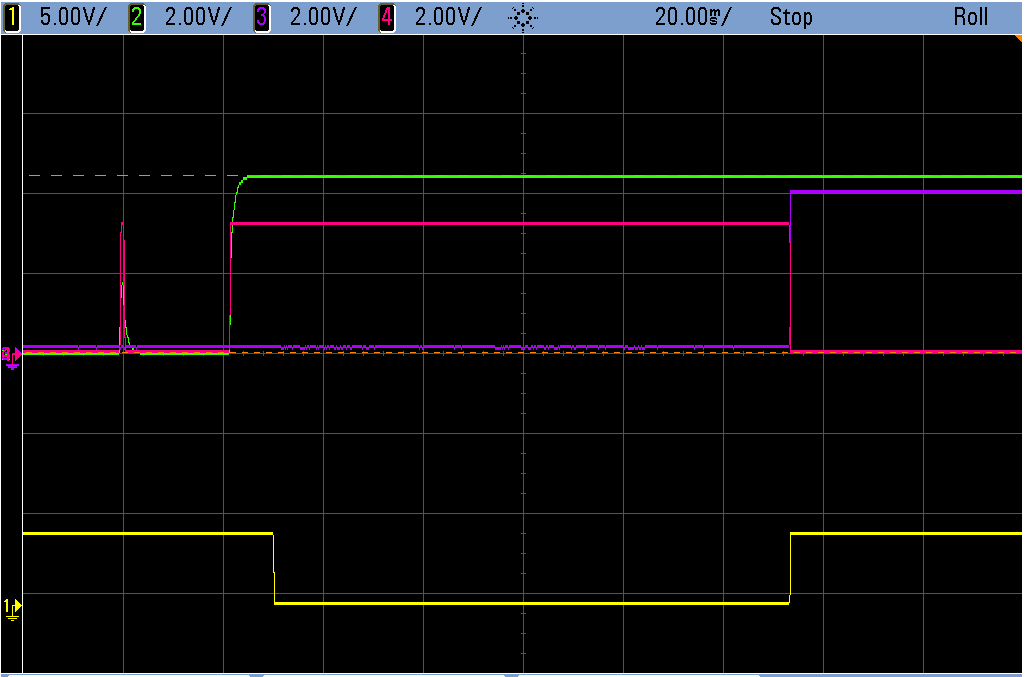
\includegraphics[scale=0.5]{../Ejercicio-3/imagenes/e3_tp3.png}
\par\end{centering}
\caption{Transisión de estados}

\end{figure}

\begin{figure}[H]
\begin{centering}
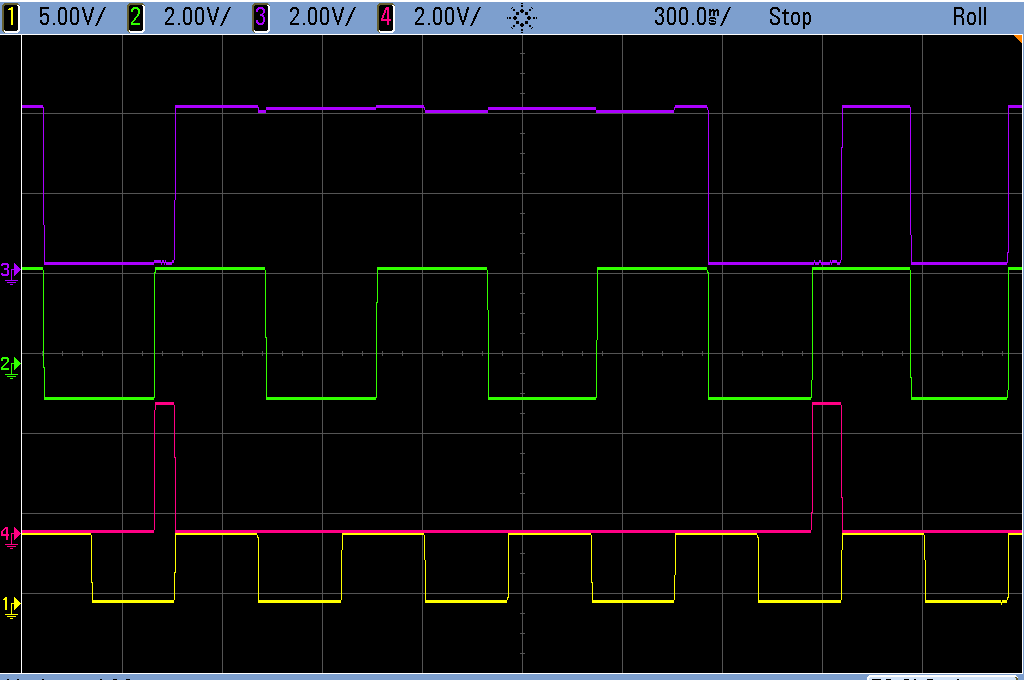
\includegraphics[scale=0.5]{../Ejercicio-3/imagenes/e3_tp3_b.png}
\par\end{centering}
\caption{Transisión de estados}

\end{figure}

En las figuras anteriores, las cuales pertenecen al circuito de Mealy, se tiene el clock como la señal amarilla, la señal de input como verde, la salida no negada del flip-flop como la violeta y finalmente la salida del circuito como rosada. Se observa al comnutar la entrada al valor HIGH en el intervalo de tiempo compendido este evento y el flanco positivo del clock se tiene que la salida del será también HIGH, regresando al valor LOW cuando se alcanza dicho el flanco positivo.

\clearpage
\section*{Appendix}
\addcontentsline{toc}{chapter}{Appendix}


\begin{thebibliography}{}
\addcontentsline{toc}{chapter}{References}
\bibitem{INT1} Stephen Brown and Zvonko Vranesic. "Fundamentals of Digital Logic with Verilog Design" third edition.
 \end{thebibliography} 
 
\end{document}
